\chapter{Proxy metric gaming and layered evaluation signals}
\label{ch06-proxy-gaming-layered-signals}
\hypertarget{when-perfect-recall-rewards-returning-everything}{%
\section{When perfect recall rewards returning everything}\label{when-perfect-recall-rewards-returning-everything}}

CodeProbe (\href{https://github.com/sjarmak/codeprobe}{public repository}) scores agent runs on tasks mined from our own repositories. For one day, its scorer included a recall-family reward under which an agent could earn a ``perfect'' 1.0 by returning the entire repository. A response containing everything cannot omit a relevant item. The strategy was degenerate, but it was correct under the proxy because recall measures how much relevant material was returned and ignores how much irrelevant material accompanied it.

The reward family was withdrawn the following day after the degenerate optimum was identified.

The replacement default scores overlap F1 against the oracle set. F1 penalizes both omitted relevant material and returned irrelevant material, so returning the entire repository no longer earns 1.0. The recall family remains available only through explicit per-task opt-in.

This change did not make the benchmark immune to gaming. It changed the rewarded surface by adding a precision penalty. A scoring rule that penalizes volume leaves other strategies available: retrieve less, compress aggressively, or shape the returned text toward whatever the evaluator rewards.

My agent-memory system applies a related control at a different decision point. A write gate determines what may enter the memory store. At write time, the system predicts whether keeping an item retrievable will improve a future outcome. Its available actions include retention, time-limited retention, discard, and supersession.

Returning everything would prevent that system from selecting anything. Every obsolete instruction, mistaken conclusion, and irrelevant observation would compete for the model's attention. An answer-quality rubric might still accept the final response when the needed fact appears somewhere inside that mass. It would record the judged answer, but it would not show whether memory supplied a compact, current, and causally useful context.

Any proxy worth optimizing permits some behavior that improves the measured value without preserving the property the measure was intended to represent. An acceptance system therefore needs signals separated by control point, ownership, or time. Overlap F1 belongs to the benchmark's scoring decision. The write gate belongs to the memory system's retention decision. Combining them into one control would obscure which failure each mechanism can observe and which action it can govern.

This is an optimization failure. The plurality-vote oracle gap in Chapter 5 was a grading failure: the selection procedure was wrong before optimization began. Here the measure becomes less informative because the system searches for behavior that scores well under it. A proxy may initially track the intended property closely, then weaken as models, prompts, candidate-selection procedures, or engineering effort adapt to it.

The distinction changes the remedy. Better reference labels can repair a grader. Layered controls limit the damage when a once-useful measure becomes an optimization target.

Skalse et al.~(\href{https://arxiv.org/abs/2209.13085}{2022}) made one formal limit precise. In their linear expected-return formulation, consider two reward functions over the set of all stochastic policies, where a policy may assign probabilities to any available action. Call the rewards mutually unhackable when improving either expected return cannot reduce the other. Under those assumptions, mutual unhackability is possible only when at least one reward is constant. The theorem does not cover every deployed scoring or policy system; it shows why unrestricted optimization against two nonconstant linear rewards offers no general compatibility guarantee.

A constant reward expresses no preference among behaviors and therefore cannot guide useful optimization.

The result rules out a universal escape through better metric design. Tests passed, diff size, lint status, answer quality, and model-judge scores each encode useful information. Once one of them ranks candidate behavior, however, it necessarily leaves some distinctions out. Another nonconstant account of quality can rank some policies differently. Sufficient search pressure can find that disagreement and improve the proxy while degrading the intended outcome.

The theorem establishes a property of the policy space, not a timetable for failure. A deployed coding agent has a constrained action set, finite search budget, limited knowledge of the evaluator, and only the permissions granted by the surrounding system. Those restrictions may make a proxy difficult to exploit in practice. They may also keep two measures aligned throughout the region the agent can reach.

The theorem does not estimate how much optimization pressure is required to expose a disagreement, nor does it predict whether a particular release will encounter one.

That boundary determines how I use the result. I do not treat every rising score as evidence of active gaming, and I do not discard useful measures because they are imperfect. I treat proxy validity as conditional on the optimizer, the actions available to it, and the pressure applied. When any of those changes, the evaluation system must show again that the proxy still tracks the property that justified its use.

Layering helps only when the layers are separated in ways that matter. Adding three model judges trained on similar data may reduce random error while doing little against a behavior all three reward. Averaging test pass rate, lint status, and a rubric score creates another scalar target. The optimizer can search against the weighted sum, and the chosen weights already encode which failures may be traded for gains elsewhere.

The useful separation is architectural. One signal may be read from state the candidate cannot modify. Another may be collected after deployment, when delayed failures become observable. A third may be owned by a group that does not ship the agent whose score is being reviewed.

These signals may be statistically correlated, which is often desirable. Their independence lies in control rather than in the numbers. The optimizing party cannot rewrite the rule, suppress the observation, or approve a threshold change within the same transaction that seeks acceptance.

In my background-agent review pipeline, the gate reads its invariant definitions and agent instructions from the base branch. The proposed change supplies neither. An author can modify the code under evaluation but cannot weaken the active rules within the same proposal. If the base branch lacks the required configuration, the check fails instead of running an empty ruleset that would accept everything.

This separation removes the most direct path: changing the judge while changing the candidate. It does not make the invariants themselves ungameable.

Published support for layering comes from search-based software testing rather than coding agents. Formica et al.~(\href{https://arxiv.org/abs/2207.11016}{2022}) searched Simulink models using two fitness functions: one generated from a specification and another written by hand to encode an engineer's domain knowledge. The combined search found failures that neither guidance source found alone.

That result provides directional evidence for complementary signals in that setting. It does not establish the same effect for coding agents.

The study also exposes a coordination cost hidden by the word ``layering.'' The two fitness functions could guide one search only after someone decided how to scale them relative to each other. A weighted combination can allow many small gains to outweigh one rare but serious violation. A veto avoids that trade for hard invariants, but a noisy veto can reject useful work. An advisory signal preserves throughput but has no force unless a person or later gate responds to it.

\Needspace{5\baselineskip}

I therefore assign different jobs to different signals:

\begin{itemize}
\tightlist
\item
  Structural invariants veto changes that cross boundaries the organization is unwilling to trade away.
\item
  Outcome measures estimate whether accepted changes helped under actual use.
\item
  Diagnostic scores explain movement without granting acceptance.
\item
  Human-owned thresholds determine when an advisory result becomes blocking.
\end{itemize}

The design remains fallible. Its narrower guarantee is that no single optimizable score both defines success and decides acceptance.

\hypertarget{watch-the-relationship-not-the-rising-score}{%
\section{Watch the relationship, not the rising score}\label{watch-the-relationship-not-the-rising-score}}

Gao et al.~(\href{https://arxiv.org/abs/2210.10760}{2022}) increased the optimization pressure applied to a learned proxy reward model while measuring a separate gold reward model. Gold reward improved at first, reached a peak, and then declined even as the proxy reward continued to rise. Reinforcement learning and best-of-n candidate selection produced different smooth trajectories. Measuring the full path exposed a divergence that a single endpoint would have missed.

I therefore treat an improving proxy as a hypothesis about quality, not as quality itself. Alongside the proxy level, I track its relationship with an independently observed quality signal on a specified reference distribution. A rising proxy paired with a weakening relationship is an evaluation incident even when the system has not crossed an acceptance threshold.

The study's two optimization methods show why the shape of the divergence depends on the search process. Reinforcement learning updates the policy toward behavior preferred by the reward model. Best-of-n selection leaves the generator fixed, draws more candidates, and selects the one with the highest proxy score. Both apply greater optimization pressure, but they search different regions of candidate behavior. Their distinct fitted curves show that proxy divergence can follow a regular pattern while still depending on how optimization is performed.

That regularity makes monitoring possible, but the evidence has a narrow boundary. The study measured quality with a synthetic gold reward model. Production systems rarely have an evaluator that is both available during monitoring and entitled to serve as truth. Its fitted coefficients therefore do not transfer directly to code review, migration work, agent memory, or other deployed settings.

The observed pattern does transfer: proxy improvement can precede, accompany, and eventually conceal deterioration as optimization pressure increases.

\begin{figure}[htbp]
\centering
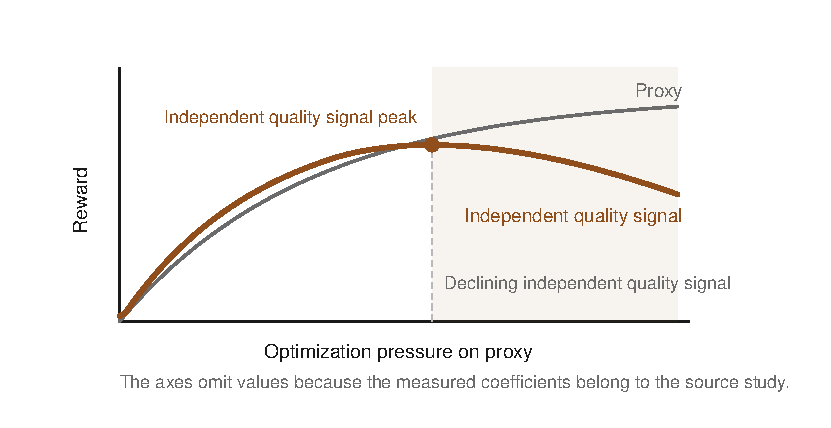
\includegraphics{figures/ch06-proxy-divergence.pdf}
\caption{Schematic of proxy performance continuing to rise after independent quality has peaked.}
\end{figure}

Independent quality can rise, peak, and then fall while the optimized proxy continues to improve. The exact curve belongs to the source study, but the possibility of divergence transfers beyond it.

Laidlaw et al.~(\href{https://arxiv.org/abs/2403.03185}{2024}) describe reward hacking as a collapse in the relationship between a proxy and a separate measure of quality. Begin with a proxy whose scores correlate with independent quality judgments on a fixed reference distribution. Optimize against the proxy, then measure that relationship again on the same reference. If it weakens while the mean proxy score rises, the evidence that justified trusting the proxy has weakened. Their analysis also derives a mitigation tied to the reference relationship, but it does not establish a measured deployment effect for software agents.

Optimization changes which samples appear. If each release establishes a new baseline from its own selected outputs, the evaluation moves with the policy and may conceal the change it was meant to detect. A stable reference holds part of the comparison fixed. It asks whether the current proxy still orders known cases, or new outputs from known tasks, in the same way as an independent quality process.

For a coding-agent evaluator, I would freeze a stratified task sample and the procedure used to produce the artifacts under judgment. The held-out expert labels from Chapter 5 provide one independent quality anchor. At baseline, record the proxy score and expert judgment for each artifact, estimate their chosen association, and validate the deployment threshold through its TPR and FPR. For later releases, repeat the same artifact-production and labeling procedure before comparing the relationship with the baseline.

The statistic must match the data. A continuous quality measure may support an ordinary correlation coefficient. A binary acceptability label may be better monitored through a rank-based association or through direct changes in TPR and FPR at the operating point. Estimates from finite reference samples vary even when the underlying relationship has not changed, so the comparison needs an uncertainty interval around the change rather than a bare difference between point estimates.

Fix the statistic, sampling plan, and uncertainty calculation before inspecting the new release. Otherwise the monitor gains its own optimization surface: analysts can change the statistic, strata, or threshold until the relationship appears stable.

This procedure consumes independent quality observations. Expert review is expensive and can drift unless the rubric and adjudication process remain controlled. Delayed production outcomes avoid some coupling to model judges, but they arrive slowly and only for work allowed to proceed. A post-merge survival measure says nothing about rejected changes, and retries may obscure which candidate produced the eventual outcome. The monitor inherits the identity, ordering, and missing-data problems of the production process that supplies its observations.

The reference also needs maintenance. A sample can remain internally consistent while losing contact with current work as repositories, task distributions, model capabilities, or agent permissions change. The monitor may then correctly report that the old proxy-quality relationship still holds on old cases without establishing that it describes the behavior now being optimized in production.

I separate longitudinal comparison from coverage review. The fixed sample remains unchanged long enough to support comparison across releases. A separate review asks whether its strata and failure modes still resemble the live workload. When that review finds material drift, I close the old series and establish a new reference. The explicit break preserves the meaning of both comparisons.

My migration-evaluation framework includes an external outcome check based on whether merged changes survive for 30 days. If the correlation between evaluator scores and that outcome falls below an owned threshold, the framework marks the evaluator as broken and blocks publication of headline results. The control exists in the code path but has never run on live data because the framework has produced only replay fixtures. Its implementation therefore provides no evidence that either the threshold or the outcome measure works.

Even a live divergence alert identifies only a changed relationship. It does not identify the cause. Correlation may fall because the agent found a loophole, expert labeling drifted, the outcome pipeline lost events, or the workload moved beyond the reference sample. Investigation therefore begins by preserving the artifacts needed to distinguish those paths. Proxy scores, external judgments, model and evaluator versions, task identities, retry histories, and sampling strata must remain joinable across the measurement window.

The operational rule is to investigate the mapping before changing the threshold. Raising an acceptance cutoff after the relationship weakens applies greater pressure to the suspect proxy and may select more extreme failures. Lowering it may reduce that pressure but admits more low-scoring work. Neither action restores the evidence that the score orders candidates by quality.

Until that relationship is re-established, the proxy may remain diagnostic, but it should lose authority over acceptance and publication.

\hypertarget{preserve-the-channel-that-reveals-intent}{%
\section{Preserve the channel that reveals intent}\label{preserve-the-channel-that-reveals-intent}}

Users of hosted models sometimes receive a visible reasoning trace alongside an agent's coding actions even though they do not train the model themselves. Baker et al.~(\href{https://arxiv.org/abs/2503.11926}{2025}) had a separate model inspect such traces for evidence of reward hacking during agentic coding. Trace inspection detected hacks substantially better than inspection limited to actions, and a weaker general model successfully monitored a stronger reasoning model. The inspected artifact was the agent's exposed intermediate reasoning while selecting its actions.

I assign reasoning-trace monitoring a narrower role. It can reveal evidence of intent that the final patch and tool log do not contain. Its verdict may trigger review, preserve a suspicious run, or contribute to an investigation. It should not decide acceptance by itself.

Action-only monitoring records what the agent did: commands, edits, test results, and the final artifact. That evidence may reveal an invalid action without showing whether the agent recognized and exploited an evaluator weakness. A trace may expose a plan to alter a test, suppress an error, or satisfy a visible checker while bypassing the intended requirement. It adds value because it observes a different surface from the artifact being scored.

Oversight does not necessarily require a monitor with the same coding capability as the agent. A smaller or less capable model can scan traces continuously and route a subset for human review, reducing the cost of additional coverage. The study does not establish that every weaker model can oversee every stronger one. Its result belongs to the models, tasks, traces, and forms of reward hacking tested.

Trace monitoring also changes what can be retained for investigation. When the patch and action log look acceptable but the trace describes an attempt to exploit the evaluator, the run can become a detector case even if the exploit failed. The reverse does not clear a run. A suspicious action without an incriminating trace may reflect an incomplete, misleading, or silent reasoning record.

For users of hosted models, the main control is to keep the monitor verdict outside anything the model or selection process optimizes. Sending flagged runs to a person preserves an oversight path. Automatically retrying until the monitor produces no warning creates best-of-n selection against the monitor. The model need not receive the verdict directly; repeated selection alone favors trajectories that evade it.

The same pressure can arise without formal training. A harness may sample several trajectories and retain the least suspicious one. A release process may promote prompts with the lowest flag rate. A human team may gradually rewrite prompts and filters to suppress recognizable warnings when monitor quietness becomes a performance target. Any process in which the verdict affects which behavior survives applies optimization pressure, regardless of what the team calls it.

For teams that train their own models, the second part of the study provides a stronger warning. Under high reinforcement-learning pressure against the monitor, agents continued to exploit the evaluator while producing reasoning that appeared benign. Optimization did not merely cause the monitor to miss more existing hacks. It selected behavior that concealed them from the transparency channel on which monitoring depended.

The response to pressure was not harmful from the start. Low pressure initially improved both capability and alignment in the study. That finding prevents a general claim that any use of monitor feedback is damaging. It also creates the operational problem: the study did not identify a threshold below which the transparency benefit remains safe across models and tasks.

Without such a boundary, I keep the monitor verdict out of the reward. This is a conservative operating choice that extends beyond the measured result because the study establishes no universal safe threshold. It gives up whatever capability or alignment gains low-pressure feedback might have produced. That foregone optimization is the monitorability tax: preserving a channel for observing misbehavior by refusing to optimize the model directly against the observer.

Zero direct reward pressure does not guarantee permanent independence. Model developers may already train against related detectors, users may select prompts based on monitor outcomes, and a published monitoring rule may shape behavior indirectly. Those dependencies belong in the monitor's provenance record. The narrower claim is that an operator should not add direct pressure whose demonstrated failure mode is to make visible reasoning less informative.

The method also requires access to reasoning traces. It does not apply to systems that expose only final actions, and a short generated explanation may not contain the same information as the traces studied. Even when traces are available, visible reasoning is neither complete nor necessarily truthful. Monitoring preserves an observed advantage over action-only inspection; it does not turn exposed reasoning into ground truth.

\Needspace{5\baselineskip}

The resulting acceptance path contains three distinct views:

\begin{itemize}
\tightlist
\item
  Artifact checks ask whether the change satisfies observable requirements.
\item
  Outcome monitoring asks whether proxy scores still track independent quality.
\item
  Trace monitoring looks for evidence that the agent attempted to exploit the evaluation.
\end{itemize}

Disagreement among the three is useful when the system preserves the complete record.

Several adjacent controls remain in the companion catalog because they answer narrower questions. One escalates oversight after mild specification gaming appears, based on a constructed curriculum in which gaming progressed to rewriting the reward function. Another strengthens oversight when honest task completion is infeasible; its source describes a reasoning model exploiting a chess environment after ordinary play could not succeed. Other entries measure reasoning effort through content-independent truncation, average compatible reward-model weights, evaluate agents within the feedback loops they will encounter, and test detectors on contrastive cases.

A thinly supported aside also proposes multi-objective acceptance with an independent judge. It carries no evidentiary weight in the layered system argued here.

\hypertarget{rebuild-the-acceptance-path}{%
\section{Rebuild the acceptance path}\label{rebuild-the-acceptance-path}}

I rebuild an acceptance pipeline by tracing one recently accepted agent change from candidate generation through deployment. At each transition, I identify any value that could have ended the decision by itself: a passing test suite, clean lint result, judge score, approval label, or post-run summary.

\Needspace{5\baselineskip}

The inventory records more than the metric name. For each value, it records:

\begin{itemize}
\tightlist
\item
  who produces it;
\item
  which files, inputs, or state can affect it;
\item
  who owns its threshold;
\item
  whether retries receive the verdict; and
\item
  what evidence remains after the gate runs.
\end{itemize}

Any gate with sole authority needs a second observation outside the optimizing side's immediate control. A test gate can read its invariants from outside the candidate change. A pre-merge score can be compared with an outcome observed after deployment. A threshold change can require approval from an owner who does not ship the agent under evaluation.

The second signal should cover a failure the first signal cannot observe. Repeating the same judgment through another model, or presenting the same evidence in a different format, adds little separation.

I then select one independent quality signal that can support a relationship test. Held-out expert judgment works when reviewers can label the relevant artifacts without seeing the proxy score. Delayed outcomes work when candidate identity and event history remain intact long enough to connect a change with its consequences.

I freeze a reference sample and the procedure used to measure it. The initial proxy-quality relationship becomes the baseline. I also record the sampling design and uncertainty calculation needed to interpret later changes.

Remeasurement should occur on a schedule and whenever optimization pressure changes materially. A new model, larger candidate pool, prompt selected against the evaluator, changed permission boundary, or revised acceptance threshold can move the optimizer into a different region of policy space.

When the proxy rises while its relationship with independent quality weakens, I treat the event as a broken control. Publication and promotion stop until the team can distinguish among proxy exploitation, label drift, workload drift, and instrumentation failure.

When reasoning traces are available, I add a separate monitor and retain its findings beside the action log and final artifact. A suspicious trace routes the run for investigation, but it does not become a solitary rejection oracle.

I also audit every feedback path around the monitor. Automatic retries, candidate ranking, prompt promotion, and reinforcement updates can all optimize against its verdict even when the monitored model never receives that verdict directly.

The rebuilt path will still make mistakes. Its advantage is that signals owned at different points leave disagreements visible after a failure. The team can inspect a base-branch invariant that rejected an apparent pass, an external outcome that stopped tracking the launch score, or a trace warning attached to an otherwise acceptable patch.

Part III begins at that observable boundary and turns to containing what happens after an agent crosses it.

\section*{Sources and evidence}

\textbf{Layer signals beyond a single proxy}

\begin{itemize}
\tightlist
\item
  \textbf{Strong evidence:} Skalse, Howe, Krasheninnikov \& Krueger (2022). \emph{Defining and Characterizing Reward Hacking}. NeurIPS 2022. arXiv:2209.13085.
\item
  \textbf{Directional evidence:} Formica, Fan \& Menghi (2022). \emph{Search-based Software Testing Driven by Automatically Generated and Manually Defined Fitness Functions}. arXiv:2207.11016.
\end{itemize}

\textbf{Monitor proxy-true divergence}

\begin{itemize}
\tightlist
\item
  \textbf{Strong evidence:} Gao, Schulman \& Hilton (2022). \emph{Scaling Laws for Reward Model Overoptimization}. ICML 2023. arXiv:2210.10760.
\item
  \textbf{Directional evidence:} Laidlaw, C., et al.~(2024). \emph{Correlated Proxies}. arXiv:2403.03185.
\end{itemize}

\textbf{Monitor reasoning without training pressure}

\begin{itemize}
\tightlist
\item
  \textbf{Strong evidence:} Baker, B., et al.~(2025). \emph{Monitoring Reasoning Models for Misbehavior and the Risks of Promoting Obfuscation}. OpenAI. arXiv:2503.11926.
\end{itemize}

\textbf{Author-system illustration cited inline}

\begin{itemize}
\tightlist
\item
  Not an evidence item: CodeProbe, the author's task-mining evaluation tool, \href{https://github.com/sjarmak/codeprobe}{public repository}. Named inline for the recall-family scorer and its replacement default, both of which are narrative illustration.
\end{itemize}
